\chapter{Rectificatifs : rapport de conception}

Nous avons fait très peu de changement sur la conception du projet par rapport au rapport. En effet, une bonne partie de l'application était alors déjà réalisée sous la forme du prototype utilisé lors de la phase de test en Décembre. Après nous êtres assurés que cette base était solide et fonctionnelle, nous avons pu continuer le développement sans rencontrer de problème majeur. 

Les seuls changements notables concernent la base de donnée. Nous avons parfois du ajouter quelques attributs à certaines entités pour permettre l'implémentation de fonctionnalités avancées (ajout d'un attribut date aux fichier uploadés par exemple, etc). La nouvelle base de donnée est représentée sur la figure \ref{bdd}.

Ces ajustements restent néanmoins mineurs dans la conception du projet.



\begin{figure}
	\centering
	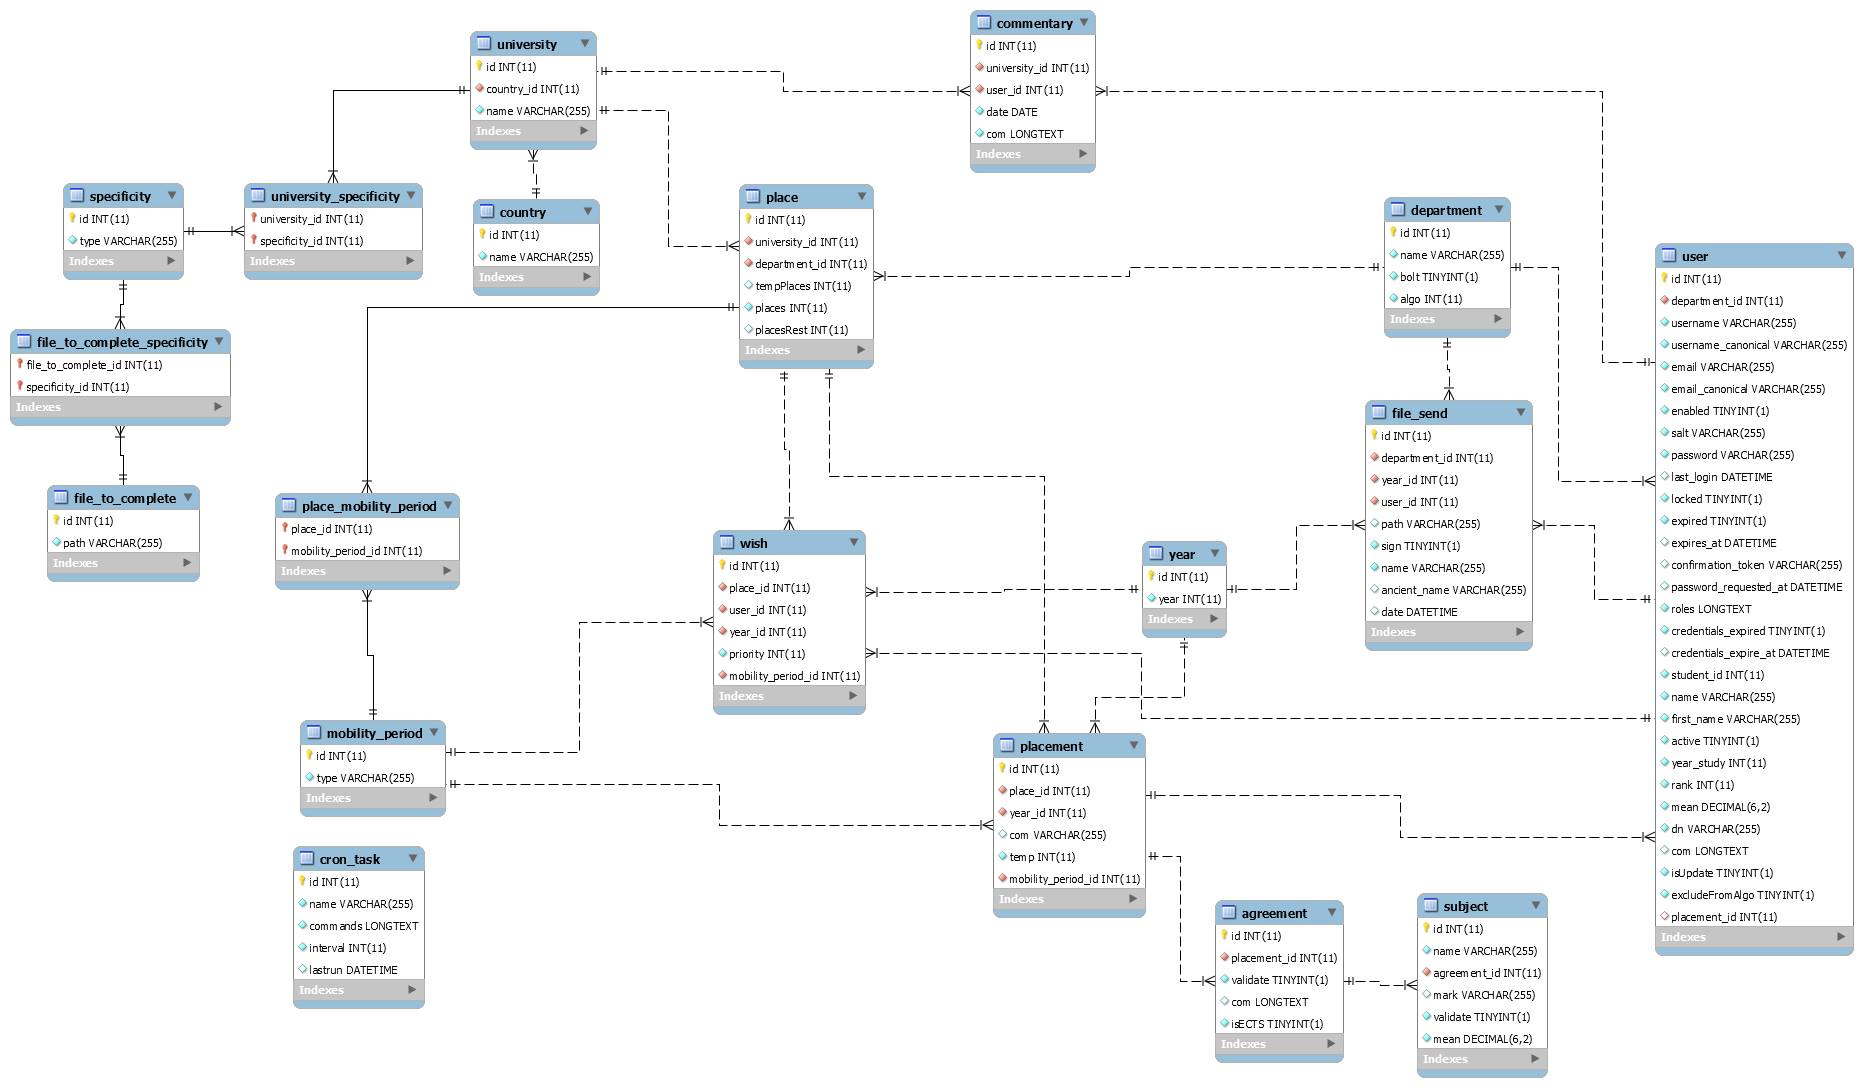
\includegraphics[angle=90,scale=0.35]{images/screen_bdd.png}
	\caption{Nouvelle base de données}
	\label{bdd}
\end{figure}

